
%%%%%%%%%%%%%%%%%%%%%%%%%%%%%%%%%%%%%%%%%%%%%%%%%%%%%%%%
%
% Copyright (c) 2003-2010 by University of Queensland
% Earth Systems Science Computational Center (ESSCC)
% http://www.uq.edu.au/esscc
%
% Primary Business: Queensland, Australia
% Licensed under the Open Software License version 3.0
% http://www.opensource.org/licenses/osl-3.0.php
%
%%%%%%%%%%%%%%%%%%%%%%%%%%%%%%%%%%%%%%%%%%%%%%%%%%%%%%%%

\section{Newtonian Potential}

In this chapter the gravitational potential field is developed for \esc.
Gravitational fields are present in many modelling scenarios, including
geophysical investigations, planetary motion and attraction and microparticle
interactions. Gravitational fields also presents the opportunity to demonstrate
the saving and visualisation of vector data for Mayavi.

The gravitational potential $U$ at a point $P$ due to a region with a mass
distribution of density $\rho(P)$, is given by Poisson's equation
\citep{Blakely1995}
\begin{equation} \label{eqn:poisson}
\nabla^2 U(P) = -4\pi\gamma\rho(P)
\end{equation}
where $\gamma$ is the gravitational constant.
Consider now the \esc general form, which can simply be related to
\autoref{eqn:poisson} using two coefficients. The result is
\begin{equation}
-\left(A\hackscore{jl} u\hackscore{,l} \right)\hackscore{,j} = Y
\end{equation}
one recognises that the LHS side is equivalent to 
\begin{equation} \label{eqn:ex10a}
-\nabla A \nabla u
\end{equation}
If $A=\delta\hackscore{jl}$ then \autoref{eqn:ex10a} is equivalent to
\begin{equation*}
-\nabla^2 u
\end{equation*}
and thus Poisson's \autoref{eqn:poisson} satisfies the general form when
\begin{equation}
A=\delta\hackscore{jl} \text{ and } Y= 4\pi\gamma\rho
\end{equation}
At least one boundary point must be set for the problem to be solvable. For this
example we have set all of the boundaries to zero. The normal flux condition is
also zero by default. For a more realistic and complicated models it may be
necessary to give careful consideration to the boundary conditions of the model,
which can have an influence upon the solution.

Setting the boundary condition is relatively simple using the \verb!q! and
\verb!r! variables of the general form. First \verb!q! is defined as a masking
function on the boundary using
\begin{python}
q=whereZero(x[1]-my)+whereZero(x[1])+whereZero(x[0])+whereZero(x[0]-mx)
\end{python}
This identifies the points on the boundary and \verb!r! is simply
ser to \verb!r=0.0!. This is a dirichlet boundary condition.

\section{Gravity Pole}
\sslist{example10a.py}
A gravity pole is used in this example to demonstrate the radial directionality
of gravity, and also to show how this information can be exported for
visualisation to Mayavi or an equivalent using the VTK data format. 

The solution script for this section is very simple. First the domain is
constructed, then the parameters of the model are set, and finally the steady
state solution is found. There are quite a few values that can now be derived
from the solution and saved to file for visualisation.

The potential $U$ is related to the gravitational response $\vec{g}$ via
\begin{equation}
\vec{g} = \nabla U
\end{equation}
This for example as a vertical component $g\hackscore{z}$ where
\begin{equation}
g\hackscore{z}=\vec{g}\cdot\hat{z}
\end{equation}
Finally, there is the magnitude of the vertical component $g$ of
$g\hackscore{z}$
\begin{equation}
g=|g\hackscore{z}|
\end{equation}
These values are derived from the \esc solution \verb!sol! to the potential $U$
using the following commands
\begin{python}
g_field=grad(sol) #The graviational accelleration g.
g_fieldz=g_field*[0,1] #The vertical component of the g field.
gz=length(g_fieldz) #The magnitude of the vertical component.
\end{python}
This data can now be simply exported to a VTK file via
\begin{python}
# Save the output to file.
saveVTK(os.path.join(save_path,"ex10a.vtu"),\
        grav_pot=sol,g_field=g_field,g_fieldz=g_fieldz,gz=gz)
\end{python}

\begin{figure}[ht]
\centering
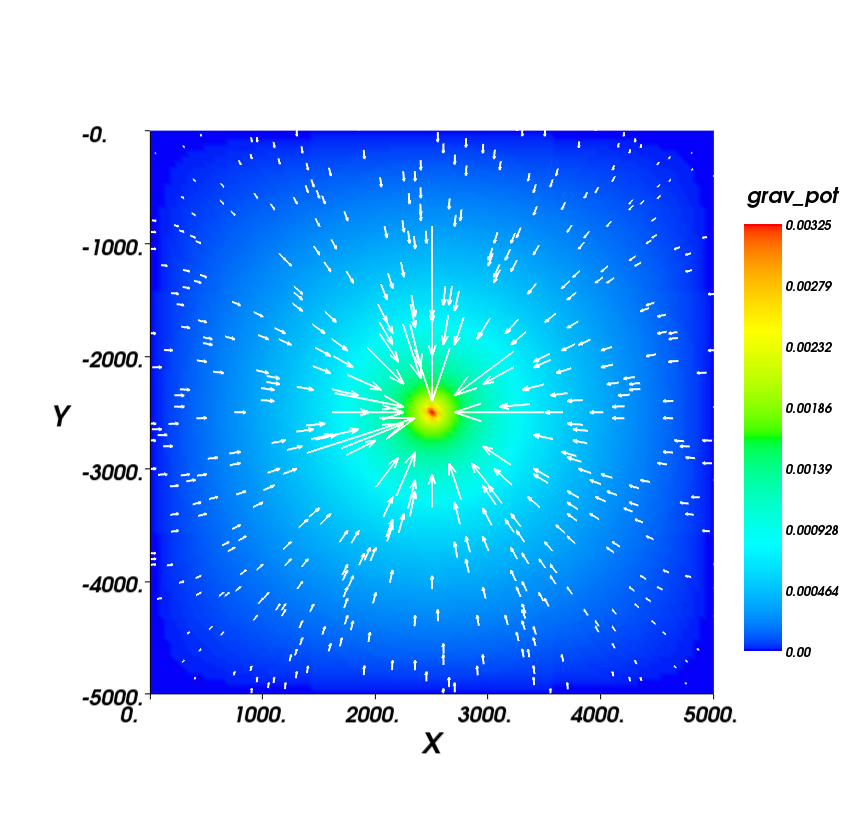
\includegraphics[width=0.75\textwidth]{figures/ex10apot.png}
\caption{Newtonian potential with g field directionality.}
\label{fig:ex10pot}
\end{figure}

\section{Gravity Well}
\sslist{example10b.py}
Let us now investigate the effect of gravity in three dimensions. Consider a
volume which contains a sphericle mass anomaly and a gravitational potential
which decays to zero at the base of the anomaly.

The script used to solve this model is very similar to that used for the gravity
pole in the previous section, but with an extra spatial dimension. As for all
the 3D problems examined in this cookbook, the extra dimension is easily
integrated into the \esc solultion script.

The domain is redefined from a rectangle to a Brick;
\begin{python}
domain = Brick(l0=mx,l1=my,n0=ndx, n1=ndy,l2=mz,n2=ndz)
\end{python}
the source is relocated along $z$;
\begin{python}
x=x-[mx/2,my/2,mz/2]
\end{python}
and, the boundary conditions are updated.
\begin{python}
q=whereZero(x[2]-inf(x[2]))
\end{python}
No modifications to the PDE solution section are required. This make the
migration of 2D to a 3D problem almost trivial.

\autoref{fig:ex10bpot} illustrates the strength of a PDE solution. Three
different visualisation types help define and illuminate properties of the data.
The cut surfaces of the potential are similar to a 2D section for a given x or y
and z. The iso-surfaces illuminate the 3D shape of the gravity field, as well as
its strength which is give by the colour. Finally, the streamlines highlight the
directional flow of the gravity field in this example.

\begin{figure}[htp]
\centering
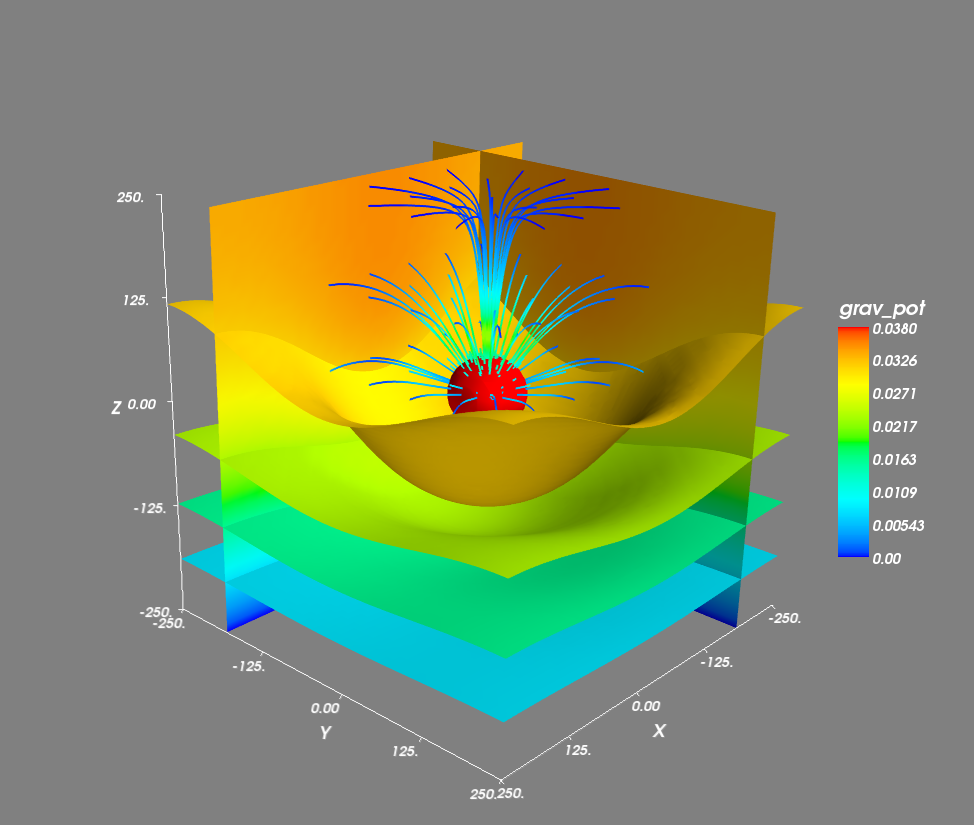
\includegraphics[width=0.75\textwidth]{figures/ex10bpot.png}
\caption{Gravity well with iso surfaces and streamlines of the vector
gravitational potential.}
\label{fig:ex10bpot}
\end{figure}

\section{Gravity Surface over a fault model.}
\sslist{example10c.py,example10m.py}
This model demonstrates the gravity result for a more complicated domain which
contains a fault. Additional information will be added when geophysical boundary
conditions for a gravity scenario have been established.

\begin{figure}[htp]
\centering
\subfigure[The geometry of the fault model in example10c.py.]
	{\label{fig:ex10cgeo}
	 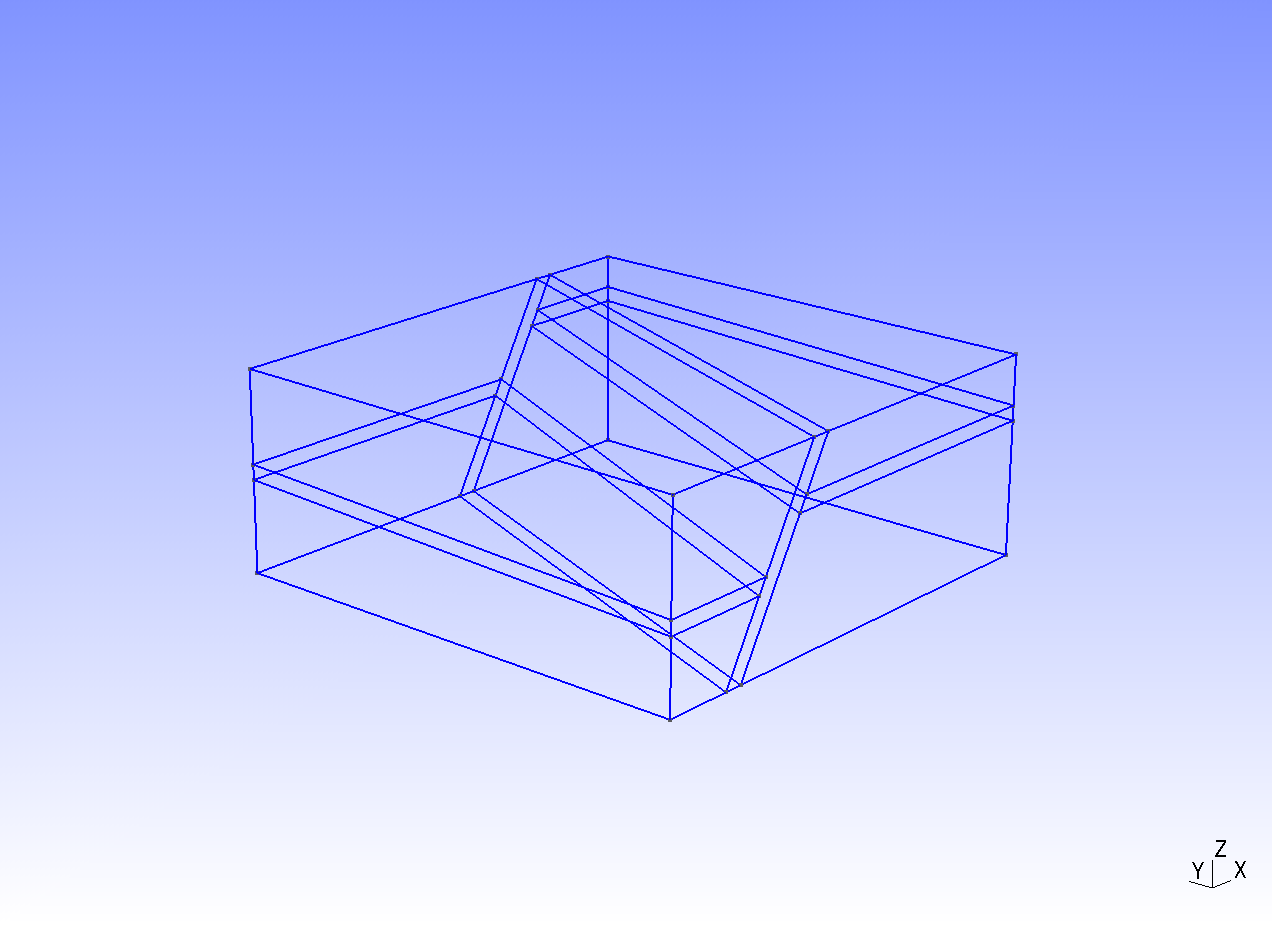
\includegraphics[width=0.8\textwidth]{figures/ex10potfaultgeo.png}} \\
\subfigure[The fault of interest from the fault model in
	example10c.py.] 
	{\label{fig:ex10cmsh}
	 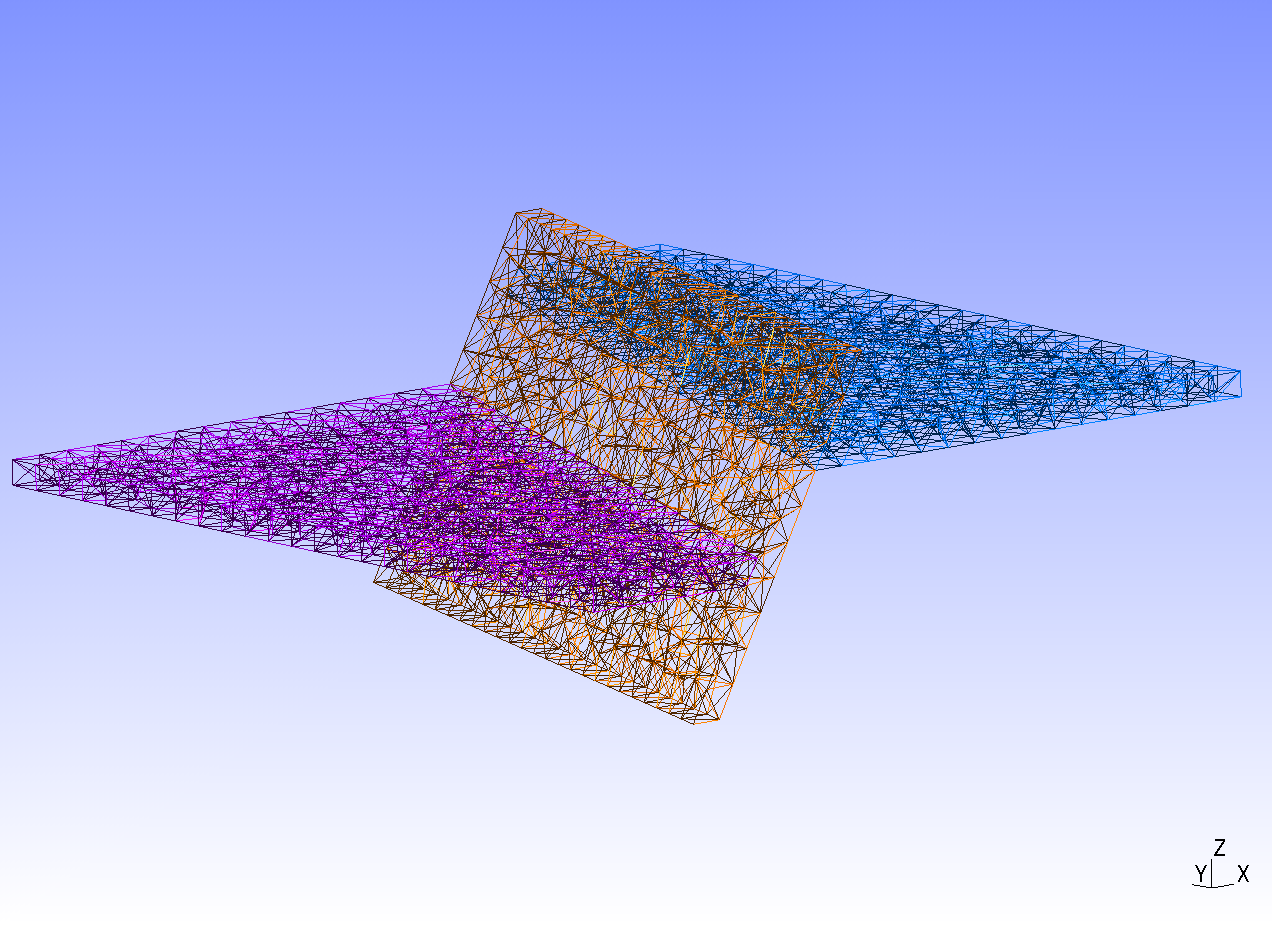
\includegraphics[width=0.8\textwidth]{figures/ex10potfaultmsh.png}}
\end{figure}

\begin{figure}[htp]
\centering
	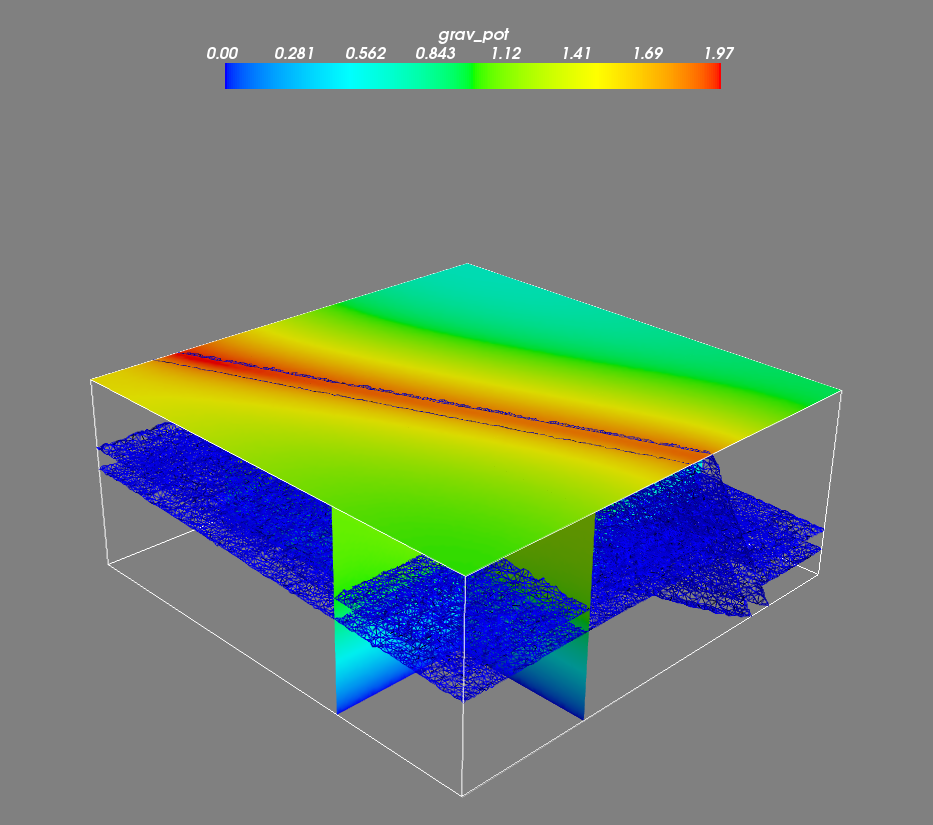
\includegraphics[width=0.8\textwidth]{figures/ex10cpot.png}
	\caption{Gravitational potential of the fault model with primary layers and
	faults identified as isosurfaces.}
	\label{fig:ex10cpot}
\end{figure}

